\documentclass[a4paper, twoside, english, 11pt]{report}
\usepackage{graphicx} 				% In order to include graphic.
\usepackage[latin1]{inputenc}		% Norwegian letters
\usepackage{url}
\usepackage{array}
\usepackage[pdftex,colorlinks]{hyperref}
\usepackage{acronym}				% All those acronyms...
\usepackage{eurofont}
\usepackage[top=3.0cm, bottom=2.5cm, left=2.5cm, right=2.5cm, bindingoffset=1cm, includefoot]{geometry}
\setcounter{secnumdepth}{3}			% The depth to which section numbering occurs
\usepackage{listings}
\usepackage{supertabular}
\usepackage{longtable}
\usepackage{multibib}
\usepackage{enumerate}
\usepackage{verbatim} 				% Inputing text files
\usepackage{courier}
\usepackage{caption}
\usepackage{wrapfig}
\usepackage{setspace}

\newcites{web}{Web References}
\hypersetup{%
		bookmarksnumbered,
		linkcolor=black, 		% Color for normal internal links.
		anchorcolor=black,		% Color for anchor text.
		citecolor=black,		% Color for bibliographical citations in text.
		filecolor=magenta, 		% Color for URLs which open local files.
		menucolor=red, 			% Color for Acrobat menu items.
		pagecolor=red, 			% Color for links to other pages
		urlcolor=blue, 			% Color for linked URLs.
}%
\setlength{\parindent}{0pt} 
\setlength{\parskip}{2ex}
\usepackage{fancyhdr}
\pagestyle{fancy}
\fancyhf{}
\fancyhead[RO]{\bfseries\rightmark}
\fancyhead[LE]{\bfseries\leftmark}
\renewcommand{\headrulewidth}{0.5pt}
\addtolength{\headheight}{0.5pt}
\addtolength{\footskip}{0.5pt}
\cfoot{\thepage} 
\pagestyle{fancy}


\begin{document}

% FRONT PAGE
\pagestyle{empty}
\begin{titlepage}
 
	\parindent=0cm
	\addtolength{\parskip}{\baselineskip}

	
\includegraphics[width=0.4\textwidth]{images/logo_ntnu.pdf}
	\vspace{2cm}\vspace{0.5cm}
	
	{\Huge \textbf{Implementing a Secure Ad Hoc Network}}

	{\LARGE Master Thesis}
	
		\vspace{1.5cm}	
		\begin{figure}[ht!]
		\centering
		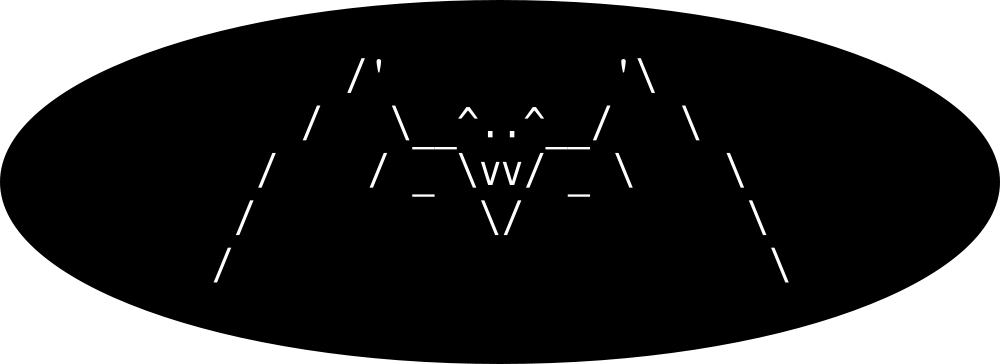
\includegraphics[width=15cm]{images/1000px_official_batman_logo.png}

	\end{figure}
	\vfill
	
	{\normalsize Trondheim, \today
	
	Norwegian University of Science and Technology\\
	Faculty of Information Technology, Mathematics and Electrical Engineering \\
	Department of Telematics}
	\vspace{2cm}\vspace{0.75cm}

	{\large Espen Grannes Graarud}

\end{titlepage}


% PROBLEM DESCRIPTION
\cleardoublepage
\pagestyle{empty}

% Latex-versjon av ITEM rapportmal.
% Lagd av <lasse.karstensen@gmail.com>, desember 2009.
% Lisens: public domain. 
%
\setlength{\parindent}{0pt} 
\setlength{\parskip}{2ex}
\begin{titlepage}
\begin{center}
\textsc{NORWEGIAN UNIVERSITY OF SCIENCE AND TECHNOLOGY\\
FACULTY OF  INFORMATION TECHNOLOGY, MATHEMATICS AND ELECTRICAL ENGINEERING} \\
\vspace{0.5cm} 
% crop-et fra http://www.ntnu.no/infoavdelingen/selvhjelp/logoer/ntnu/NTNU_engelsk_RGB.png

\includegraphics[scale=0.5]{images/NTNU_logo.png} \\

\vspace{1.0cm}
{\Huge{PROBLEM DESCRIPTION}}
\vspace{1.0cm}

\begin{tabular}{ p{4cm} p{11cm}}

Student:	& Espen Grannes Graarud \\
Title: & Implementing a Secure Ad Hoc Network \\\\
%\vspace{1cm}
Description: & \\
\end{tabular}
{\small{\begin{tabular}{p{15cm}}
\vspace{0.2cm}
 
B.A.T.M.A.N. is a pro-active routing protocol for ad hoc networks that is
designed to be a simpler and more robust alternative to the OLSR protocol. The
project work of Anne Gabrielle Bowitz and Espen Graarud proposed to add routing
message authentication in B.A.T.M.A.N. using proxy certificate mechanisms.
\\\\
This thesis work will determine the performance of this secured protocol
in comparison with the original B.A.T.M.A.N protocol, for instance by
measuring network convergence time. Tests should also be run to find how the
secure protocol protects against known attacks such as the wormhole attack.


\end{tabular}  }}

\begin{tabular}{ p{4cm} p{11cm}}
Deadline: & June 29, 2011\\
Submission date: & \today\\
Department: & Department of Telematics\\
Supervisor: & Stig Frode Mj{\o}lsnes, ITEM\\
Co-Supervisor: & Martin Gilje Jaatun, SINTEF\\
 & Dr. Lawrie Brown, UNSW@ADFA\\\\
\end{tabular}
\vspace{0.5cm}

Trondheim, \today 

\vspace{1cm}
\line(1,0){190} \\
Stig Frode Mj{\o}lsnes, NTNU ITEM

\end{center}
\end{titlepage}



\cleardoublepage
\pagenumbering{roman}			% Roman numbers in the beginning of the report is nice.
\pagestyle{fancy}

% ABSTRACT
\cleardoublepage
\chapter*{Abstract}
\addcontentsline{toc}{chapter}{Abstract}

%In emergency situations and military operations it is useful to be able to
%quickly establish communication. It is often necessary to accomplish this with
%minimum pre-existing infrastructure and without centralized administration. In
%such scenarios it would also be important that the network is secure - not only
%implying keeping the communication secret, but also be able to restrict access
%to the network. Wireless ad hoc networks fulfill many of these requirements,
%but the issue of security and access control still remains a challenging task.
%\\\\
%The goal of this study can be divided into two parts. The first part was
%focused on trying to define a system with a proper authentication scheme that
%does not affect the nature of ad hoc networks. We combined common
%authentication mechanisms and an ad hoc routing protocol for this purpose.
%Secondly, the B.A.T.M.A.N. routing protocol was extended to incorporate the
%very basic functionality of the system design proposed.
%\\\\
%A small laboratory environment was set up to test the performance of the
%extended protocol with the intention of proving that our basic functionality
%did not weaken the unique properties of mobile ad hoc networks. The test
%results shows that the basic idea of our system design is possible, and that
%the current implementation should be further extended to fulfill the
%requirements necessary for a secure ad hoc network.

\pagestyle{empty}					% In order to remove the black line on the top. Unfortunately the page number is also removed...

% PREFACE
\cleardoublepage
\pagestyle{fancy}
\chapter*{Preface}
\addcontentsline{toc}{chapter}{Preface}

This master thesis is written by Espen Grannes Graarud and concludes my 5
year master programme in Communication Technology specializing in Information
Security at the Norwegian University of Science and Technology, NTNU.

This thesis is a continuation of my and Anne Gabrielle Bowitz' Information
Security specialization project that was proposed by Dr. Lawrie Brown of
UNSW@ADFA, Australia, and Martin Gilje Jaatun of SINTEF ICT, Norway.

I would like to thank my fellow student Anne for our great co-operation during
the project and for her thoughts and ideas during the writing of this thesis. I
would also like to thank my supervisors, especially Martin for his great weekly
feedbacks which was a great help along the way.

Finally I would like to thank my responsible Professor Stig Frode Mj{\o}lsnes
from the Department of Telematics at NTNU for his feedback on the system design.

\begin{center}
\vspace{4cm}
\noindent Trondheim, \today
\vspace{2cm}
\\Espen Grannes Graarud
\end{center}


% ABBREVIATIONS
\clearpage
\chapter*{Acronyms}
\addcontentsline{toc}{chapter}{Acronyms}

\begin{acronym}

\acro{3G} {3rd Generation Mobile Telecommunications}

%\acro{AC} {Attribute Certificate}

\acro{AL} {Authentication List}

\acro{AM} {Authentication Module}

\acro{BATMAN} {Better Approach To Mesh Ad hoc Networking}

\acro{CA} {Certificate Authority}

\acro{CBC} {Cipher-block Chaining}

%\acro{CRL} {Certificate Revocation List}

%\acro{DHCP} {Dynamic Host Configuration Protocol}

%\acro{DNS} {Domain Name System}


\acro{ECC} {Elliptic-Curve Cryptography}

\acro{EEC} {End-Entity Certificate}

\acro{IV} {Initialization Vector}

\acro{LLPKC} {Long-Lived Public-key Certificates}

\acro{MAC} {Message Authentication Code}

\acro{MANET} {Mobile Ad Hoc Network}

%\acro{MPR} {Multipoint Relay}

\acro{NL} {Neighbor List}

\acro{OASIS} {Open Advanced System for dISaster and emergency management}

\acro{OGM} {Originator Message}

\acro{OLSR} {Optimized Link State Routing}

\acro{OSI} {Open Systems Interconnection}

\acro{PC} {Proxy Certificate}

\acro{PC0} {Proxy Certificate 0}

\acro{PC1} {Proxy Certificate 1}

%\acro{PKC} {Public Key Cryptography}

\acro{PKI} {Public Key Infrastructure}

%\acro{SLC} {Short Lived Certificates}

%\acro{SLCS} {Short Lived Credential Service}

\acro{SP} {Service Proxy}

\acro{SSO} {Single Sign-On}

\acro{TTL} {Time To Live}

%\acro{UAV} {Unmanned Aerial Vehicle}

\acro{Wifi} {Wireless Fidelity (See '802.11' in Definitions)}

\acro{WOT} {Web Of Trust}

\end{acronym}


% DEFINITIONS
\clearpage
\chapter*{Definitions}
\addcontentsline{toc}{chapter}{Definitions}


%TODO: Change to some other package. COnflicts with actual acronyms list.
\begin{acronym}
%Legg inn i alfabetisk rekkefølge!

\acro{802.11}
	IEEE 802.11 standard, wireless, more more

\acro{Ad Hoc Network}
	A self-organizing network with no form for pre-existing infrastructure or
	centralized administration.

\acro{Asymetric Link}
	If traffic is only possible in one direction, i.e. a node can receive but not
	send packets to another node, the link in between them is called an asymetric
	link.

%\acro{Authenticated List} %egendefinert forkortelse av espen
%	A list containing the public keys, IP, roles, certificate validity period,
%	signature fraction and the timestamp of the last received signature of all
%	authenticated nodes in the network. The list broadcasted by the SP
%	periodically.

\acro{Authentication}
	Say something about authentication

\acro{Authentication Module}
	Addition to the B.A.T.M.A.N. protocol which takes care of cryptographic
	functions and other additions. It also adds fields to the Originator messages
	which can contain a digital signature or signature fractions, and sends other
	messages with nonces, certificates, and ALs.

\acro{Authentication Token}
	Say something about authentication tokes, such as certificates and so on\ldots

\acro{Authorization}
	Say something about authorization

\acro{Congestion}
	Congestion is a state in wich the the amount of traffic on a network surpasses
	the stable amount of traffic the network can handle. I.e. congestion can make
	the network useless if not handled by some control mechanisms.
	
\acro{Certificate Authority}
	Say something about CAs.

%\acro{Convergence Time}
%	The time it takes for the network to get to a stable state with no route
%	flapping after an event that has changed the network topology. E.g. a node has
%	died or moved and made a link inferior to other alternative links.

\acro{Elliptic-Curve Cryptography}
	Public key cryptography based on the mathematical properties of elliptic
	curves.

\acro{End-Entity Certificate}
	A X.509 public key certificate of an end user.

\acro{Link-local}
	See Neighbor.

%\acro{Multicast}
%	In computer networking this refers to the delivery of a packet or message to a
%	group of devices.

\acro{Neighbor}
	Neighbor refer to actual link-local a neighbor, i.e. a node within
	transmitting range for which you can communicate directly with.

\acro{Originator}
	Synonym for a Batman interface which is a network interface utilized by
	Batman.

\acro {Originator Message}
	Batman protocol message advertising the existence of an originator. They are
	used for link quality and path detection \cite{batman_rfc}. %CP

%\acro{Packet Delivery Ratio}
%	Proportion of delivered packets relative to the amount of packets sent.

\acro{Pro-Active Routing}
	TODO

\acro{Proxy Certificate} 
	A X.509 certificate signed by a regular X.509 EEC. It is used to assign roles
	to which the recipient can act on behalf of the signee.

\acro{Proxy Certificate 0}
	Say something about PC0
	
\acro{Proxy Certificate 1}
	Say something about PC1
	
	
\acro{Public Key Infrastructure}
	Every entities involved with the management (creation, distribution etc.) of
	public key certificates. Managed by the PKIX working group of IETF.

%\acro{Round Trip Delay}
%	The time it takes from a packet is sent from the sender and the sender
%	receives as acknowledgment packet from the receiver.

\acro{Route Flapping}
	Occurs when a node in a network continuously changes preferred route between a
	source and destination pair creating route instability.


\acro{Routing Protocol}
	TODO

\acro{Service Proxy}
	Say something about SPs.

%\acro{Shortest Path}
%	Minimum number of hops between two communicating nodes.

\acro{Socket}
	Say something about sockets.

\acro{Thread}
	Say something?

\acro{Web Of Trust}
	GnuPG project\ldots

\acro{X.509 Certificates}
	Standard public key certificate standard managed by the PKIX working group of
	IETF.

\end{acronym}


% TABLE OF CONTENTS, LIST OF FIGURES AND LIST OF TABLES
\tableofcontents
\listoffigures
\listoftables
\pagestyle{empty}	

% INTRODUCTION
\cleardoublepage
\pagenumbering{arabic}			% Arabic numbering. Starts on page 1 again.
\pagestyle{fancy}
\chapter{Introduction}
\label{ch:intro}
\acresetall
We have become accustomed to an almost complete presence of digital networks
in our daily lives. Everywhere you go, you can either plug your laptop into an
ethernet slot, connect your iPad to an available wifi hot spot, or just use
your cell phone via 3G mobile data network. However, this is not universally
true throughout the world. Many places are sparsely populated, or the people
living there do not have the resources to deploy such networks.

In emergency and/or military situations, this often applies. Even if it didn't,
the networks may have been put out of operations due to the nature of the
emergency (i.e. tsunami destroying the infrastructure). As recent events
here in Norway have shown, internal errors might paralyze the whole network 
infrastructure\footnote{\url{http://www.dagbladet.no/2011/06/16/nyheter/innenriks/telenor/16942385/}
(Norwegian)} making emergency relief ineffective\footnote{\url{http://www.dagbladet.no/2011/06/11/nyheter/ver/flom/naturkatastrofer/innenriks/16880835/}
(Norwegian)}, giving a sound argument for having a separate backup emergency
network. The military might also be in an hostile environment where they cannot trust
the network in place altogether.

Emergency search and rescue and military tactical operations can greatly benefit
from the use of digital communication for sharing operation critical
information. If they have no trusted data network available, they should
therefore set up one themselves. A realistic approach would have to be easy and
quick to set up and be self-managing, thus requiring minimal maintenance. It
should to an extent always be available to the participants wherever they go,
which calls for using a wireless network. Last but not least, the network needs
to be trusted, i.e. you should trust that the infrastructure is not compromised
and that the communicating parties on the network are who they claim to be.

A \ac{MANET} solves some of these requirements. It does not need an existing
communication infrastructure, it is self-organizing and the network coverage
range can easily be extended by placing intermediate nodes in strategic
locations. The latter requirement however, is a more challenging task in
\acp{MANET}.

With the lack of infrastructure in \acp{MANET} and no guarantees that they are
connected to the Internet, establishing trust between the nodes becomes
different from how this is done on the Internet which can rely on e.g.
\acp{PKI}.

In this thesis I will propose and implement a solution suggestion to establish a
trust mechanism, i.e. an authentication scheme, which combines features of a
typical \ac{PKI} with some of the ideas behind \ac{WOT}
\cite{zimmermann1995official}. The system design is presented in two parts, the
part which has been implemented in Chapter \ref{ch:design}, and the ideas that I
did not have time to implement are discussed as further work in Chapter
\ref{ch:discussion}.

As one might expect, it is a very challenging task to achieve strong security
for \acp{MANET} and still have the benefits of its simple ``plug and play''
design. As real world implementations go, there are a few trade-offs, and
security cannot always win. This design will not try to be 100\% secure, but
should be secure enough to deploy in emergency situations. To back this claim,
the Norwegian Army recently stated that their new computer security guidelines
is to rather have a usable (available) system which might be open to attack,
instead of a bad system which is impenetrable - as long as they are able to
monitor and take action against potential
attacks\footnote{\url{http://www.tu.no/it/article287598.ece} (Norwegian)}.

\section{Motivation}
The 7.0 magnitude earthquake that struck Haiti in 2010 showed us how huge
relief efforts easily become very inefficient when huge amounts of emergency
relief personnel work at a scene with little or scarce communication throughout
the area\footnote{\url{http://www.wired.com/magazine/2010/04/ff_haiti/}}. With
a trusted communication network like a secure \ac{MANET} an operation like this
could become much more efficient, bringing the right amount of help to the
right places at the right time.

\section{Contributions}
This thesis presents a novel design to achieve authentication and trust
between nodes in a secure ad hoc network. The popular ad hoc routing protocol
called BATMAN has been extended to become an instantiation of said design, which
has never been done before. Additionally, the use of proxy certificates for
trust establishment for ad hoc networks is also a novel approach to the problem.

\section{Objectives}
The main objective of this thesis is to design and implement an authentication
extension to ad hoc networks based on a known routing protocol.

Secondly, other design ideas, or things that was supposed to be in the design
but did not make the time frame is discussed upon in contexts of both security
and real world performance.

Last, but not least, testing of the proposed design's implementation should be
done to compare the performance of the new implementation against the original
routing protocol.

The problem description also mentions testing the implementation against known
security attacks. However, my responsible Professor Stig Frode Mj{\o}lsnes
claimed no such tests were necessary as the security of this design should
rather undergo peer review and testing, therefore these tests have not been
done.

\section{Limitations}

\subsection{IP Address Configuration}
\label{limit:ip_address_conf}
Autoconfiguration of network interfaces for ad hoc networks is a huge and
difficult task and will not be addressed in this thesis. Throughout this thesis
the assumption is that all nodes trying to participate in the same network is
pre-configured with a valid and unique IP on the correct subnet. It is also
assumed their network interfaces are correctly set up to connect to the correct
wireless channels.

\subsection{Detecting malicious behavior}
\label{limit:malicious_behaviour}
One attack vector which will not be discussed in this thesis is if a legitimate
node acts maliciously, which might happen if a legitimate node is compromised.
The solution proposed in the thesis assumes all trusted nodes acts with good
intentions. There are much research about detecting malicious behavior in ad
hoc network \cite{Pirzada_McDonald} \cite{dhurandher2010network}.

However, these kind of solutions are mainly designed for networks without any
authentication scheme at all, and is therefore just investigating malicious
behavior without trying to detect whether a node is compromised or not. These
proposals might therefore not be of the greatest interest, but should be studied
to see if any of their features can safely be applied to an ad hoc network with
an authentication system in place.

\section{Method}
The primary research method conducted in this thesis is the \emph{design
science paradigm} for Information Systems research as described in
\cite{hevner2003information}. The model and method artifacts of this paradigm
are described in Chapter \ref{ch:design} whereas the instantiation artifact is
described in Chapter \ref{ch:implementation}.

Much of the design (method artifact) comes from the specialization project last
fall \cite{bowitz_graarud}, but some aspects of that design has been changed
during the course of the study and implementation in this thesis.

\section{Document Structure}
This thesis report is structured as follows:

\textbf{Chapter \ref{ch:background}: Background} aims to give the reader the
necessary insight about the technologies, ideas and theories discussed later in
this thesis.

\textbf{Chapter \ref{ch:design}: System Design} proposes an original solution
for an authentication scheme for \acp{MANET}.

\textbf{Chapter \ref{ch:implementation}: Implementation} presents the
implementation of the system design. The implementation is a modification of the
\ac{BATMAN} source code.

\textbf{Chapter \ref{ch:testing_results}: Testing \& Results} devise different
tests for checking the performance of the implementation compared to the
original \ac{BATMAN} implementation, and presents the results of the tests.

\textbf{Chapter \ref{ch:discussion}: Discussion} looks at some of the possible
vulnerabilities in the proposed design, talks a little about the experience of
implementing such a system, and takes up issues regarding extending the proposed
system design even further.

\textbf{Chapter \ref{ch:conclusion}: Conclusion} makes conclusions about the
security, and performance of this system as well as how well it fulfills the
requirements for the implementation.

\textbf{Appendix \ref{appendix:source}: Source Code} shows a few of the most
necessary code snippets and links to the full source code available online.

\textbf{Appendix \ref{appendix:lab_setup}: Lab Setup} shows how the machines
used in the lab and tests were set up.

\textbf{Appendix \ref{appendix:paper}: Scientific Paper} about adding security
to the BATMAN protocol written by myself, Anne Bowitz, and our supervisors
Martin Jaatun and Dr. Lawrie Brown.


% BACKGROUND
\chapter{Background}
\label{background}
This chapter provides the necessary background required to read and understand this report. Section \ref{ad_hoc_network} describes ad hoc networks, their unique characteristics and challenges they might introduce. The chapter then continues to explain how routing is done where two different ad hoc routing protocols are used as examples. The last section \ref{authentication} gives a short overview of different authentication mechanisms common for computer networks.

%\section{Related work}
%Some work has been done previously when it comes to developing and implementing a secure and restricted ad hoc network. Amongst them worth mentioning... blablabla
%Secure Routing for Mobile Ad hoc Networks
%A Performance Comparison of Multi-Hop Wireless Ad Hoc NeWork Routing Protocols
%Secure Extension to the OLSR protocol


\section{Ad Hoc Network}
\label{ad_hoc_network} 
Definition: \textit{``A self-organizing communications network with no form of pre-existing infrastructure or fixed centralized administration.''}
\\\\
A wireless ad hoc network is a collection of nodes able to communicate with each other by together creating and organizing a network. The network is able to perform regular network functions like access and routing without there being any pre-existing, fixed and centralized infrastructure. Thus nodes are not only end-entities, but must also be able to act like a router by forwarding traffic that is not destined to it self. %skriv bedre!
\\\\
The nodes participating in an ad hoc network can either be fixed or mobile. Ad hoc networks where the nodes are mobile, are often referred to as Mobile Ad hoc Networks (MANETs). A closely related variant of the MANET is the mesh network where the nodes are not very mobile or not mobile at all, but they can however still join or leave the network at will making the behavior of the network similar to that of a MANETs. In this report we will focus on ad hoc networks where the participating nodes can be highly mobile, thus when the term ad hoc network or just network is used, we refer to MANET unless otherwise stated.

\subsection{Applications}
\label{ad_hoc_applications}
Because of ad hoc networks self-organizing nature they need very few pre-conditions in place for establishing and maintaining a network. Thus deploying an ad hoc network can be less demanding and very quick compared to other communications network like a traditional computer network \cite{murthy-ad}. Due to ad hoc networks' special characteristics they may find applications in several areas as briefly described below.
\\\\
In emergency situations such as during war or after natural disasters, entire infrastructure-based communication may be destroyed and restoring communication quickly is crucial. By using an ad-hoc network, communication could be set up almost immediately and could then be used in emergency operations such as crowd control, search and rescue, coordinate rescue operations and so on.
\\\\
Military applications also benefit from ad hoc networks ability to form a communication network quickly. In addition to this, military operations usually require a high level of security not only by encrypting the data being transmitted, but also restricting the access to the network.
\\\\
The type of communication required in the environments mentioned above enforces other important requirements on ad hoc networks, such as reliability, efficiency, and support for multicast routing \cite{murthy-ad}. These scenarios will also be covered and further explained in chapter \ref{scenario_requirements}.
\\\\
Other areas of use for ad hoc networks are wireless sensor networks and collaborative and distributed computing \cite{murthy-ad}.

\subsection{Challenges and Issues}
\label{ad_hoc_challenges}
Despite the many of advantages that ad hoc networks may introduce, several challenges and issues are also present that affect the design, deployment, and performance of such networks. Amongst the major issues relevant for our project, we find:
%\cite{misic2008wireless}, \cite{sheu2005handbook} and \cite{murthy-ad}:

\begin{itemize}
\item Mobility of nodes
\item Unreliable medium
\item Resource constraints
\end{itemize}

\noindent
High mobility of nodes in ad hoc networks results in frequent path breaks, packet collisions, transient loops and route flapping. This causes the network topology to change randomly and frequently making it highly dynamic. Hidden and exposed terminal problems may also appear as a consequence of the mobility of the nodes. A good routing protocol should however efficiently solve or reduce the impact of such issues \cite{murthy-ad}.
\\\\
In wireless and especially in noisy wireless areas, data packets can and will get lost. In addition, ad hoc networks with only one wireless communication interface have to cope with self-inflicted interference caused by their own wireless traffic. Thus communication links may have varying quality in terms of packet loss and will therefore also affect the network topology \cite{batman_rfc}.
\\\\
All the issues mentioned above will in turn also affect the security in ad hoc network as explained in the next section.

\subsection{Security Issues}
\label{adhoc_security}
Security in ad hoc networks is a challenging and comprehensive task. The unique characteristics of these networks introduce situations that are not common to traditional computer networks. 
\\\\
Computer networks are infrastructure-based communications networks where there exists important central entities that are necessary in order to have a functional network, e.g. routers, gateways etc. These are points in the network where it is natural to place security mechanisms. However, since ad hoc networks do not have any central entities, there are no well defined points where these mechanisms could be applied \cite{murthy-ad}.
\\\\
Nodes that participate in an ad hoc network can frequently join and leave at any point in time. If there is no authentication mechanism present, there is no association or relationship between nodes and networks making it easy for an intruder to join a network and carry out an attack \cite{murthy-ad}.
\\\\
Unlike wired networks, the communication in wireless ad hoc networks is done on a shared radio channel and may easily be picked up by any node that is in range of direct transmission. A malicious node is therefore able to perform security attacks ranging from passive eavesdropping to active message replay, and message distortion \cite{806983}.
\\\\
Other aspects of ad hoc networks that may affect the security, is the limited resource availability found in such networks. Mobile nodes typically have limited computation capacity, battery power and scarce bandwidth which makes it difficult to implement computation-intensive tasks like complex cryptography-based security mechanisms \cite{1269716}.
\\\\
Different types of security attacks possible in ad hoc networks can be found in all the layers in the OSI model \cite{kurosecomputer}. Some examples of attacks that can be found in the network layer are wormhole, blackhole, Byzantine, information disclosure and routing attacks. On the transport layer we can find attacks like session hijacking. In addition there are attacks which could occur in any layer, such as Denial of Service (DoS) and impersonation \cite{murthy-ad}.

\section{Ad Hoc Routing}\label{ad_hoc_routing}
As explained in \cite{murthy-ad} the responsibilities of a routing protocol include exchanging route information, finding a good path to a destination, discovering dead links, and restoring the paths. 
\\\\
Because of ad hoc networks' unique nature, classical routing protocols are typically not well suited. Thus several routing protocols have over the years been developed specifically for ad hoc networks and they can be categorized into different groups based on their properties.
\\\\
In the sections below, two ad hoc routing protocols will be described and discussed. First out is OLSR which is a common and widely used protocol tailored for ad hoc networks \cite{zafar2008using}. The second routing protocol is BATMAN which was developed as an alternative for OLSR.

\subsection{Optimized Link State Routing protocol}
Optimized Link State Routing protocol (OLSR) is a proactive routing protocol which means that the routing in the network is done based on routing information that is periodically exchanged between nodes. The protocol belongs to the family of classical Link State Protocols which is one of two broad categories of routing protocols used in packet switching networks \cite{clausen2003rfc3626}.
\\\\
OLSR is tailored for mobile ad hoc networks by optimizing the link state protocol in two ways \cite{murthy-ad}: 

\begin{itemize}
\item reducing the size of control packets sent in the network.
\item reducing the number of links that are used for forwarding link state packets.
\end{itemize}

\noindent
These optimizations are realized by using only selected nodes, called Multipoint Relays (MPR), to retransmit control messages and link-state updates sent in the network. Every node in the network, called a Multipoint Relay Selector, chooses a set of neighboring nodes as their MPRs. The protocol uses hop-by-hop routing where only local information is used to route packets. This information is retrieved from the MPRs that periodically announce link-state information and control traffic to their MPR selectors. The basic layout of any packet that is transmitted in OLSR is shown in Figure \ref{fig:olsr}.

\begin{figure}[ht]
	\centering
		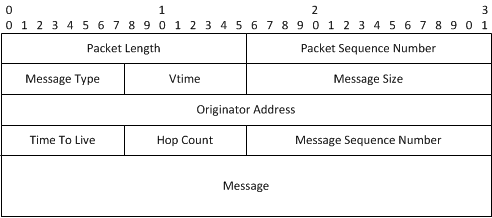
\includegraphics{images/olsr.png}
	\caption{OLSR packet format omitting the IP and UDP headers.}
	\label{fig:olsr}
\end{figure}

\noindent
Because of the regular transmission of control messages, the protocol is sustainable to packet loss which is common in wireless networks. Overhead of control messages in the network is also reduced and redundant control traffic is eliminated by using the MPRs \cite{clausen2003rfc3626}. However, because of the many optimizations added to make the protocol more suitable for ad hoc networks, it also is more complex than e.g. the BATMAN protocol explained in the section below.

\subsection{B.A.T.M.A.N.}\label{batman}
B.A.T.M.A.N., or BATMAN as we will continue to write, is an abbreviation for a "Better Approach To Mobile Ad hoc Networking". It was created with the hope of being a simpler, better and more robust alternative to OLSR. The initial motivation to start the development of the protocol was mainly based on the following reasons \cite{open_mesh}:

\begin{itemize}
\item The OLSR protocol seemed not to be very functional when implemented as specified in \cite{clausen2003rfc3626}. %RFC3626

\item The OLSR protocol depends heavily on the assumption that every node in the network is in possession of almost the same information as all of the other nodes. As they use this information to calculate full routing path to all nodes, the more this information between the nodes differ amongst them, the more likely things like routing loops will occur.
\end{itemize}

\noindent
In order to implement functional OLSR protocol to be used in real-life, the developers found themselves stripping it down removing mechanisms that were initially added to the protocol to optimize it. Eventually the developers had to break compatibility with the protocol defined in \cite{clausen2003rfc3626}. A group of developers felt the OLSR protocol was becoming far to complex and decided develop a routing protocol that was simpler and better, namely BATMAN.
\\\\
BATMAN is, as well as OLSR, a proactive routing protocol where every node has a routing table containing all of the nodes in the network that are accessible via single-hop or multi-hop communication links. The table, which is referred to as Originator List, does however not include the full path to a destination, only the best link-local neighbor towards it. Link-local neighbors are usually referred to as direct neighbors in the BATMAN protocol.
\\\\
Nodes in the BATMAN network build their Originator Lists based on Originator Messages (OGM). These messages are small, containing only a limited amount of information such as version, Time-To-Live (TTL), sequence number, some flags and an Originator Address. The Originator Address is the IP-address of the Originator where the OGM was generated. An Originator is defined in \cite{batman_rfc} as a network interface utilized by BATMAN. Every node in the network periodically generates and broadcasts OGMs for each interface it can communicate through. These messages will be re-broadcasted through the network according to BATMANs forwarding rules until they have reached all the nodes at least once. The format of an OGM is shown in Figure \ref{fig:ogm}.

\begin{figure}[ht]
	\centering
		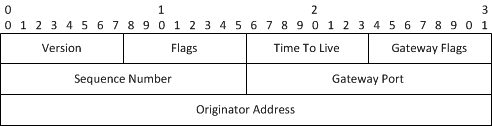
\includegraphics{images/ogm.png}
	\caption{Originator Message (OGM) Format.}
	\label{fig:ogm}
\end{figure}

\noindent
\\\\
The best route to a certain Originator is found by counting the number of OGMs received containing this Originator Address and logging which neighbor it was received from. The best route is thus the link-local neighbor that has the highest count.
\\\\
Details about the BATMAN protocol can be found in the Appendix \ref{appendix_batman}.

\subsection{B.A.T.M.A.N. and OLSR Comparison}\label{batman_olsr_comparison}
One major difference between BATMAN and OLSR is that while OLSR works to reduce the traffic load in the network by restricting which nodes that are allowed to flood, BATMAN does not care about this at all. The reasoning behind this decision is because the protocol was designed to function on unreliable media which is very unstable and can suffer from high packet loss. Thus the flooding of routing information will not saturate the network since most of the packets will be lost due to the lossy media \cite{batman_rfc}.
\\\\
In addition, the nodes in a BATMAN network do not have to calculate the full routing path to all other nodes in the network. By only choosing the next hop towards a destination makes BATMAN a lightweight protocol that quickly adapts to the dynamic topology of ad hoc networks.

\section{Authentication Using Certificates}\label{authentication} % Ny tittel!? authentication and access control / certificates / x.509 certificates
In order to have a restricted ad hoc network there needs to be some form of access control mechanism in place. In traditional computer networks the issue of access control and authentication is usually solved with the use of a hierarchy of trusted third parties, and digital certificates which is associated with every entity participating in the network. A certificate contains information about the entity that defines its identity and rights in the network.
\\\\
This section describes some of the different variants of the X.509 certificates that are used in X.509 Public Key Infrastructure (PKI). 

\subsection{X.509 Long-Lived Public-Key Certificates} \label{LLPKC}
In a Public Key Infrastructure (PKI) the conventional digital certificates are sometimes called Long-Lived Public-key Certificates (LLPKC). They are issued to end-entities by a well-known and trusted Certificate Authority (CA) that digitally signs the certificates with its private key such that it can be verified by anyone in possession of the CAs public key. Each certificate contains the public key of an end-entity and additional data such as subject's public key information, signature algorithm identifier and issuer name \cite{stallings2006cryptography}. 
\\\\
The certificate also contains a validity period of usually months or years which is why they are referred to as "Long-Lived Certificates". This long lifetime entails that a certificate needs to be checked against a Certificate Revocation List (CRL) to ensure that it has not been made invalid whilst still in its validity period. Figure \ref{fig:LLPKC} shows an illustration of a service verifying an end-entity's LLPKC and checking it against a Certificate Revocation List.

\begin{figure}[ht]
	\centering
		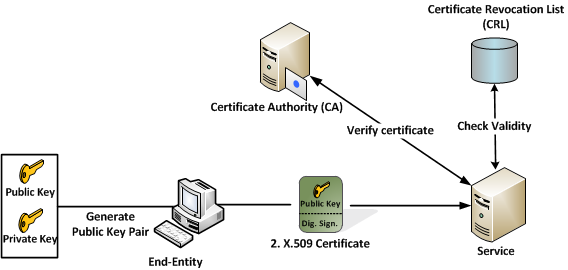
\includegraphics{images/LLPKC.png}
	\caption{An conceptual illustration of the authentication process using LLPKCs.}
	\label{fig:LLPKC}
\end{figure} 

\subsection{X.509 Proxy Certificates} \label{background_pc}
A X.509 Proxy Certificate (PC) is a conventional X.509 public-key certificate containing a critical proxy certificate information extension. The presence of this extension indicates that the certificate is a PC and that it contains one required and two optional fields; pCPathLenConstraint, proxyPolicy and Proxy Certificate Path \cite{tuecke2004rfc3820}.
\\\\
The policy field in the extension can be used to make the PC a Restricted Proxy Certificate (RPC). It contains a field which specifies the appropriate language in which the policy is expressed. This option was intended to provide a finer granularity of control in the rights being delegated.
\\\\
A PC inhabits some of the following properties as described in the Internet standard \cite{tuecke2004rfc3820}:

\begin{itemize}
\item It is signed by an X.509 End Entity Certificate (EEC), or by another PC and is called a Proxy Issuer (PI).
\item An EEC can give certain rights and restrictions to the PC it signs. 
\item It can sign another PC, but nothing else.
\item It contains its own unique public and private key pair.
\item It can be created with any desired lifetime.
\end{itemize}

\noindent
An important feature of the PC is that it is given a unique identity derived from the end-entity who signed it. During the signing the PC may also inherit rights from the PI, subject to the restrictions that are placed on that PC by the PI. Thus the PC has a unique identification which can be used independently and still be associated with the PI who signed the certificate.


\subsection{Other Certificates}
Other variants of the X.509 certificate worth mentioning are Attribute Certificates (AC) and Short-Lived Certificates (SLC). ACs are certificates with a similar structure as a LLPKC, but without a PKC key pair. They contain a set of attributes tied to an identity which is used for authorization and access control decisions. ACs are usually used in association with another certificate that do contain a PKC key pair, such as a LLPKC. The AC may have any validity period desired by the issuer and is usually has a shorter lifetime than LLPKC \cite{farrells2010rfc5755}.
\\\\
The SLCs are modified versions of the traditional X.509 certificates and differ from these mainly because of two characteristics: certificate validity period is no more than 1 million seconds and there is no association between the client and Public Key cryptography (PKC) key pairs \cite{hsu2002intranet}. They were introduced by \cite{hsu2002intranet} with the goal of reducing the costly and difficult key management issues in typical X.509 authentication framework.














% IMPLEMENTATION
\chapter{Implementation}

The security additions to the BATMAN protocol are mostly implemented in the
\ac{AM}, but some alterations had to be made in other parts of the code as well.
This chapter is devoted to explain what have been done as to achieve the design
goals, but the code itself is found in Appendix \ref{chapter_source_code}.

\section{Proof of Concept Solution with Dedicated Socket}
Based on the implementation done in the previous project where we proposed a
proof of concept solution with no actual cryptographic authentication scheme -
this section describes how that solution was extended to use a separate socket
in order to achieve the performance needed, as discussed in the project.


% Laboratory Environment and Testing
\chapter{Testing \& Results}
\label{ch:testing_results}
\acresetall

In this chapter two tests are described and their results presented and
discussed. The two tests measure and compare the time performance in two common
stages for both the original implementation of BATMAN, and the extended version
proposed and implemented in this thesis.

\section{Test I - Initialization Phase}
The ``initialization phase'' is the setup phase between two or more nodes trying
to create a network. With the original implementation of BATMAN this phase only
consist of two stages; namely discovering a neighbor node, and deciding to add
the node as a direct link, or ``last-hop'' per BATMAN terminology, in its
routing table.

With the proposed design and implementation from this thesis, two more stages
are added. After the discovery, the authentication handshake stage and the
keystream sharing stage are conducted before the last stage where BATMAN adds
the node as a new direct link in its routing table.

The time measured here in this test is the time between the first discovery of a
new neighbor, until that node is added to the routing table.

\subsection{Hypothesis}
With the modified version of BATMAN proposed in this thesis, one should observe
a small extra delay in the setup of the network, compared to the original
BATMAN protocol. This extra delay should however, not be significantly higher,
i.e. it should be relatively constant and at no time should any linear increase
in delay be observed.

\subsection{Setup}
\begin{figure}[h]
	\centering
	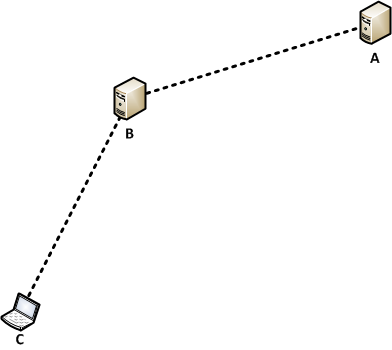
\includegraphics[width=0.5\textwidth]{images/setup_test_1.png}
	\caption{Physical network layout used in test 1. When using the modified version node B acts as the SP of the network}
	\label{fig:setup_test_1}
\end{figure}

Figure \ref{fig:setup_test_1} presents the setup of the test machines used to
conduct this first test. Node A and B are stationary boxes while node C is a
laptop. Their hardware specifications are described in Appendix
\ref{appendix:lab_setup}. The reasoning to use a different hardware for node C
is the need to create distance in the network, and that outside the ethernet
subnet for which the two other nodes were connected to, it would be easier to
use a laptop during setup. In the next test, this laptop is yet again moved
further away.

An important feature to notice about how these nodes were set up is that node A
and C are outside each other transmitting range, meaning they need an
intermediate node to route their packets to and from each other. Node B is
conveniently placed with almost equal distance to each of the two other nodes.

The landscape the nodes are setup in is a typical office landscape, with varying
obstructing materials such as concrete, wood, and glass. A more ideal setup
would naturally be outdoors, as the network is intended for, but with the lack
of mobile nodes and time this became out of the option.

\subsection{Procedure}
In order to get the same behavior each run for the modified version, each run
had to be run discretely, i.e. after each run the daemon was shut down and
restarted. This way each run will include all four stages explained above:
discovery, authentication handshake, keystream material sharing, and routing
table update. This was also done on the original implementation, even though
there are no authentication steps in between, but in order to have the exact
same procedure each time.

For each run, these steps were followed:
\begin{enumerate}
  \item Start Node A and C
  \item Wait and make sure both nodes are stable
  \item Start Node B
  \item When both node A and C are discovered and added to routing table kill
  all daemons
  \item Record the log from node B
\end{enumerate}
These steps were taken 10 times in order to have a reasonable data set and
average. Then for each of the 10 logs, record the time between the first routing
announcement received from a node, until both nodes have been added to the
routing table.

\section{Test II - Route Convergence}
The next test is to check how quick route convergence the protocols deliver when
a path between nodes in the network changes. As with the previous test, a
node running the original protocol needs to discover a new direct neighbor and
add it to its routing table. In addition, it will have to receive not only the
neighbors own routing announcements, but also routing announcements it has
forwarded on behalf of its own direct neighbors. When this happens, the node
receiving these re-broadcasts determines new routes to possibly new nodes -
adding them to its routing table.

Additionally, nodes using the modified BATMAN protocol needs to share
their keystream material with their new direct neighbor before adding that
neighbor in their routing table. When this has happened, any re-broadcasted
routing announcements from that neighbor is accepted and paths to those nodes
are updated, or added if new nodes. Note also that no authentication handshake
or sharing of certificates are mentioned, as they are assumed to have been
shared prior to this route change.

\subsection{Hypothesis}
As before, a small and relatively constant (mathematical term) extra delay is
expected when running the modified version of the protocol compared to running
the original. As the keystream material sharing only occurs between the direct
neighbors, it should only happen once during one run and not for each of the new
nodes added by the path through the direct neighbor - i.e. there should be no
linear increase in convergence time even if multiple new nodes are added to the
routing table with paths through a new neighbor.

\subsection{Setup}
\begin{figure}[h]
	\centering
	\subfloat[Initial Position - D out of range of C]{\label{fig:test_2_1}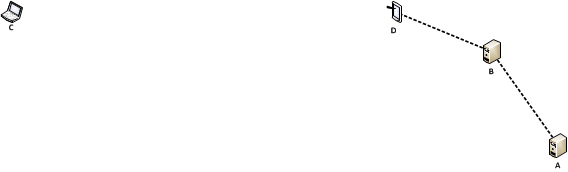
\includegraphics[width=\textwidth]{images/setup_test_2_1.png}}
	\\
	\subfloat[``Connected Position'' - D within range of C]{\label{fig:test_2_2}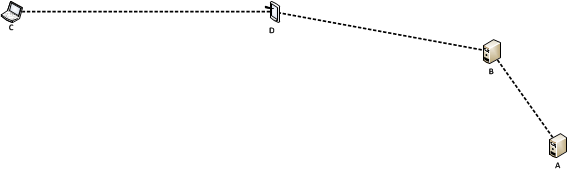
\includegraphics[width=\textwidth]{images/setup_test_2_2.png}}
	\caption{Physical network layout used in test 2. The Laptop (node C) is moved further out of range and is periodically rejoining the network when a Tablet Pc (node D) is moved within range. When using the modified version node B acts as the SP of the network}
	\label{fig:setup_test_2}
\end{figure}

For this test a new mobile node was needed. As Figure \ref{fig:setup_test_2}
shows the Laptop, or node C, from the previous test is moved much further away,
so far in fact the newly added Tablet Pc, node D, needs to place itself with
approximately the same distance to node B as to node C in order for node C to
take part in the network.

Node A and B is positioned at the same place as in the previous test, in the
same office landscape. The line of sight is, however better between node B and
D, and between D and C. Their line of sighs are only obstructed by a single wall
with huge windows.

\subsection{Procedure}
With this test running each of the 10 iterations discretely would be too time
consuming, because it would have meant that the Laptop (node C) would have to be
physically moved inside the transmitting range of node B for each run. Instead
the laptop was only started within the range of the other nodes, in order to be
authorized and share certificates with the other nodes (only node B and D was
necessary) and then moved to its position long outside the transmitting range of
the rest of the network. After this ``initial setup'' plus some minutes to
clear the neighbor lists, these steps were followed:
\begin{enumerate}
  \item Walk node D in between node B and C
  \item Wait until the whole network has stabilized
  \item Walk node D back out of node C's range
  \item Wait until BATMAN has cleared node D from other nodes routing tables,
  and node D has cleared all other nodes from its routing table
  \item If modified version is used, make also sure node D is removed from the
  \ac{NL} (should be before routing tables are cleared)
\end{enumerate}
These steps were repeated 10 times for both implementations. The records used
from this test are from the logs of node C. The convergence times measured
are the time between each time a new neighbor (node D) is discovered by BATMAN,
and until a path to the furthermost node (A) is added to the routing table.


\section{Results}
In this section the results from the two tests above are presented and discussed
in terms of how they perform compared to the hypotheses. In both tests there
were only a dataset of 10 trials, which given the variance shown below does not
provide a statistical significant result. However, the first test shows good
indication that the modified protocol behaves as expected, while the results
from the seconds test are more ambiguous. The results below are presented in
graphs, while all of the numerical results and the test logs are found in
Appendix \ref{appendix:test_results}.

\subsection{Initialization Phase}
Figure \ref{fig:results_test_1} presents the first test's results for both the
original and modified version of BATMAN. The two graphs shows the time in
seconds on the y-axis and the trial/run number on the x-axis. The two colored
lines on the graphs shows the results from first neighbor discovery until the
first neighbor is added to routing table (green line) and until both nodes are
added to the routing table (red line).

\begin{figure}[h]
	\centering
	\subfloat[Original B.A.T.M.A.N.]{\label{fig:test_1_original}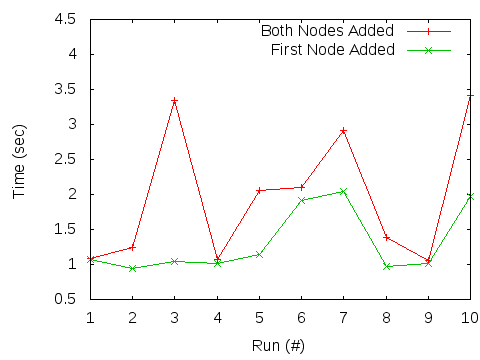
\includegraphics[width=0.5\textwidth]{images/test_1_original.png}}
	\subfloat[Modified B.A.T.M.A.N.]{\label{fig:test_1_secure}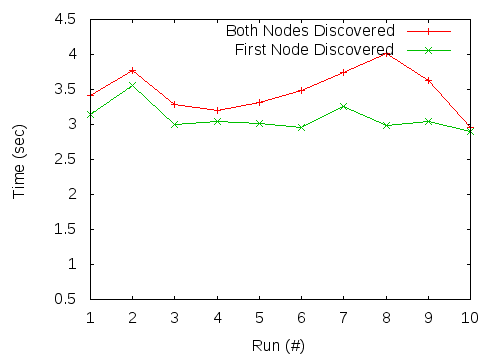
\includegraphics[width=0.5\textwidth]{images/test_1_secure.png}} 
	\caption{In a network of three nodes, the time spent by the \ac{SP} from its first neighbor discovery and until both neighbors are added to its routing table.}
	\label{fig:results_test_1}
\end{figure}

The results from the original protocol, shown in Figure
\ref{fig:test_1_original}, shows high variance in the time needed to add one and
two nodes to the routing table. For 7 out of 10 ``first nodes'' the time needed
is relatively equal, being about one second. For both nodes to be added however,
there are much more variance - varying from the best possible time, i.e. equal
to adding one node, and up above 3 times longer than adding one node. As this is
from the original implementation of BATMAN, this thesis will not try to explain
why this behavior is observed, nor does the author know exactly why either.

Figure \ref{fig:test_1_secure} shows the results from the modified version
proposed in this thesis. These results indicates that the behavior of the
modified version seems to correlate with the behavior expected from the
hypothesis. A seemingly constant of about two seconds seems to be added to the
process of adding both nodes to the routing table. 

Another interesting observation is that the time variance seems to be much less
from that of the original version. This might be because the authentication
handshake and the keystream sharing happens in a separate thread from the
regular BATMAN operations, meaning the BATMAN protocol continuously receives
routing announcements to process while the \ac{AM} handles its part. The idea
being that while the \ac{AM} thread runs the BATMAN thread ``gets ready'' to do
its part of the job.

\subsection{Route Convergence}
The results of the second test is shown in Figure \ref{fig:results_test_2}. In
this figure, the axes are the same as in the figures above: y-axis shows the
time in seconds, and the x-axis shows the trial run. The red line shows the
performance of the original implementation, while the green line shows the
modified.

\begin{figure}[h]
	\centering
	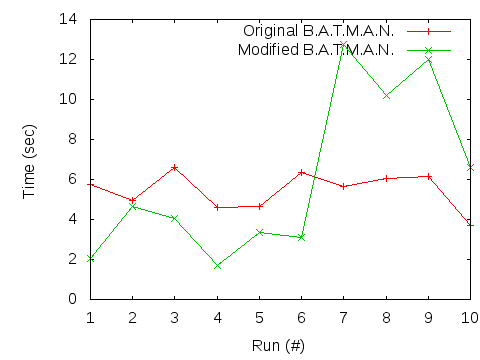
\includegraphics[width=0.8\textwidth]{images/test_2.png}
	\caption{Routing path convergence time observed by a distant source node to another sink node in the network. The source node is only sporadically connected to the network through a mobile intermediate node.}
	\label{fig:results_test_2}
\end{figure}

As indicated earlier, this test's results are somewhat unclear. While the
results using the original implementation seems relatively uniform, with only
about 1 second variance, the results from the modified implementation is highly
irregular.

Looking through the logs from this test one thing become apparent. With
different hardware on the different nodes in the network, their wireless cards
send at different strengths meaning while one node can receive packets from a
``stronger node'', the packets sent might not be received by the other nodes.

The BATMAN protocol messages (routing announcements) are sent quite often,
depending on the number of re-broadcasts being sent, meaning the time from when
a node is within transmitting range and until its broadcasts are received by
nodes within its transmitting range will be quite short. The \ac{AM} messages
however, was mostly tested in an ideal environment where most packets were
received, so this was not properly accounted for. Therefore, if a routing
announcement from a ``stronger node'' is received by a ``weaker node'', the
weaker node might send its keystream material without the other node receiving
it.

Re-transmitting mechanisms based on guessing that the receiving node has not
received the \ac{AM} messages are in place, but as the mechanism wait until it
believes the other node has not received, instead of knowing it instantly. This
can of course be managed adding ACK'ing to each \ac{AM} message, which was not
added initially because of the wish to minimize overhead. This however, might
have to be re-evaluated.

Another thing to notice is how multiple trial runs using the modified version
actually performed better than the original version. This is impossible to
explain talking about the design and implementations themselves, but is probably
most accurately explained in the terms of external environment.

In this test, one major factor is the movement of the Tablet Pc, or node D. This
movement is not perfect, and will vary in speed, timing, and accurate position
for each run. As self-generated routing announcements are only generated once
every second, a difference in almost two seconds can be seen based on the
difference in distance each run. Also, the original implementation only starts
its whole neighbor discovery after an original (self-generated/produced)
routing announcement is received from a new neighbor. The \ac{AM} is triggered
on the first routing announcement received from that new neighbor, even if that
announcement is a re-broadcast from another node in the new neighbor's network.


% RESULTS
\chapter{Results}

\section{Performance}
\subsection{Secure Implementation}
\subsection{Original Implementation}

\section{Attack Tolerance}
\subsection{Wormhole Attacks}

% CONCLUSION
\chapter{Conclusion}
\label{ch:conclusion}
\acresetall



% BIBLIOGRAPHY
\clearpage
\addcontentsline{toc}{chapter}{Bibliography}
%\nocite{*}
\bibliographystyle{alpha}
\bibliography{ref}

%\clearpage
%\addcontentsline{toc}{chapter}{Web References}
%\nociteweb{*}
%\bibliographystyleweb{plain}
%\bibliographyweb{ref}

% APPENDIX
\clearpage
\appendix
%\chapter{BATMAN Protocol}
\label{appendix_batman}
This appendix contains some additional details about the BATMAN ad hoc routing protocol.

\section{Originator Message (OGM) Format}
The core algorithm in the BATMAN protocol as well as its implementation have gone through several evolutionary changes during development. Currently the BATMAN developers are working on a version V of the protocol where they aim to improve issues such as mesh bonding, weighted Link Quality (LQ) measurements and multicast optimizations \cite{open_mesh_v}.
\\\\
During development there has also been some changes to the Originator Message (OGM) format. Figure \ref{fig:ogm} shown in Section \ref{batman} is the OGM as it is described in the Internet-Draft \cite{batman_rfc}. Two fields, Previous Sender Address and Transmit Quality (TQ), have been added to the OGM as shown in Figure \ref{fig:app_ogm}.
\\\\
A BATMAN packet consisting of an Originator Message (OGM) together with zero or more HNA extension messages, is encapsulated in a single UDP data packet. The format of the OGM is shown in Figure \ref{fig:app_ogm}.

\begin{figure}[ht]
	\centering
		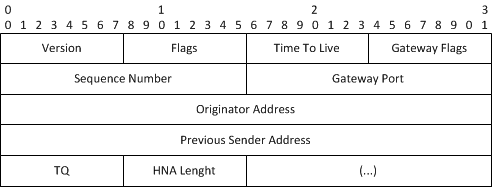
\includegraphics{images/ogm_v2.png}
	\caption{Originator Message (OGM) Format.}
	\label{fig:app_ogm}
\end{figure}

\noindent
The different fields in the OGM is explained below:
\\\\
\textbf{Version} \\
Identifies the version of BATMAN for the contained message
\\\\
\textbf{Is-direct-link flag} \\
Flag indicating whether a node is a direct neighbor or not.
\\\\
\textbf{Unidirectional flag} \\
Flag indicating whether the neighboring node is bidirectional or not.
\\\\
\textbf{Time To Live} \\
Contains the maximum number of hops a message will be transmitted.
\\\\
\textbf{Gateway Flags} \\
Indicates whether a node may act as a gateway with access to the Internet. 
\\\\
\textbf{Sequence Number} \\
Number added by an Originator to every OGM it broadcasts. Number is incremented for each OGM broadcasted.
\\\\
\textbf{Originator Address} \\ 
The IPv4 address of the B.A.T.M.A.N. interface on which behalf the OGM has been generated.


\subsection{Host Network Annoncement Message Format}
The Host Network Announcement (HNA) is used to announce that a node is a gateway to another network. If so, the node sets the Gateway Flag in the OGM and appends a HNA-extension-message containing the netmask and the network address of the announced network.
\\\\
HNA-extension-message format is shown in Figure \ref{fig:app_hna}.

\begin{figure}[ht]
	\centering
		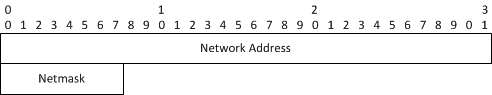
\includegraphics{images/hna.png}
	\caption{Host Network Announcement Message format.}
	\label{fig:app_hna}
\end{figure}



\end{document}
